% !TEX root = ../main.tex
% !TEX spellcheck = en_GB

\chapter{Analysis}
This section describes the analysis of the system; how the system is envisioned to be created, which subsystems it will consist of and the tasks each subsystem has to be able to perform to meet the specified requirements.

To fulfil the specified requirements in \nameref{chap:requirements} a module to locate the system, save the location and send the location must be present. Additionally a processor is needed to facilitate communication between the modules. This system interfaces with a server as shown in \cref{fig:BDD:unspecified}

\begin{figure}[H]
	\centering
	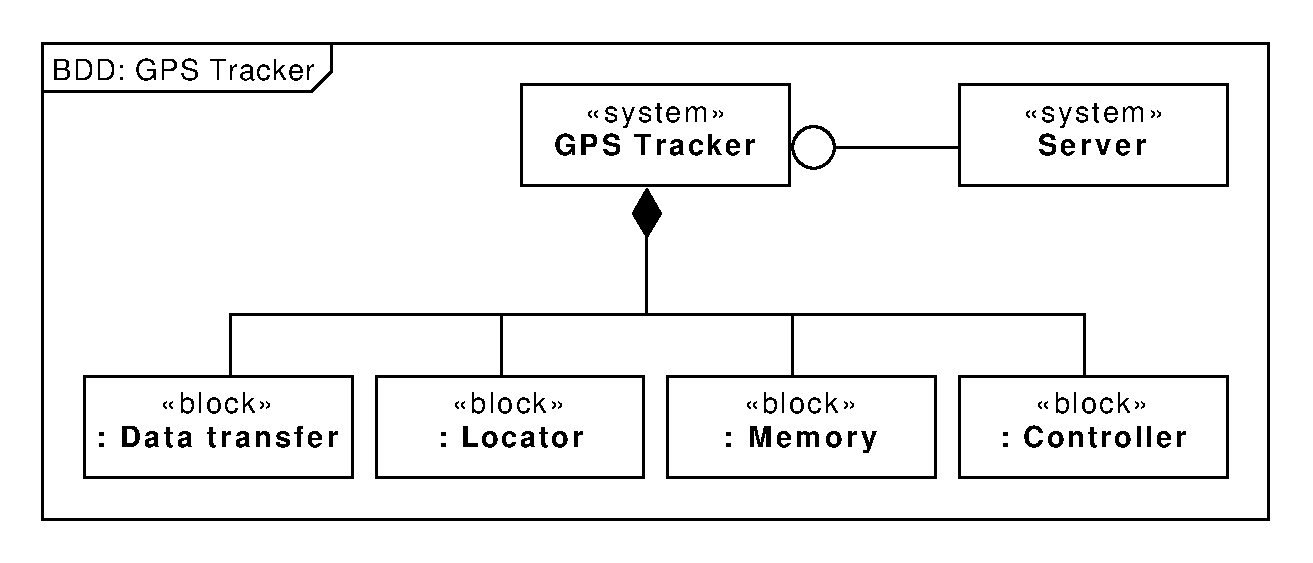
\includegraphics[width=0.7\linewidth]{gfx/Design/BDD_Unspecified.pdf}
	\caption{A high level BDD showing the parts of the \systemName, and the interface with a server.}
	\label{fig:BDD:unspecified}
\end{figure}

\section{GSM - AT Command Interface}
In order to communicate with the GSM module, it is likely that an AT interface will be used, as this has become the standard way of interaction with GSM modules.
Going through \fxnote{Reference for PDF} a range of commands has been found, that will likely be used to set up the connection and send data through UDP.

\begin{table}[H]
	\begin{tabularx}{\textwidth}{l X X}
		\toprule
		Command & Description & Chapter \\
		\midrule
		+CCID & Sim card identification. Used for checking if the sim card is recognized. & 4.12 \\
		+CSQ & Check signal quality. & 7.2 \\
		+COPS & Operator selection and status. & 7.4 \\
		+CGDCONT & Connection settings and apn. & 18.4 \\
		+CGATT & GPRS attach or detach. & 18.14 \\
		+CGACT & Activate or deactivate context. & 18.16 \\
		+CGREG & GPRS network registrations status & 18.27 \\
		+USOCR & Create a socket				& 25.3 \\
		+USOST & Send UDP Datagram through socket. & 25.11 \\
		\bottomrule
	\end{tabularx}
	\caption{Table of potential AT commands to use.}
	\label{tab:ATcomm}
\end{table}

\FloatBarrier
